\documentclass[1pt]{article}
\usepackage {tikz}
\usetikzlibrary {arrows,automata}
\usepackage{amssymb}
\usepackage{listings}
%block scheme
\usepackage{pdfpages}
\usepackage{caption}
%preamble
\usepackage[nottoc]{tocbibind}
\usepackage[T1]{fontenc}
\usepackage{graphicx}

\usepackage{amsmath}

\def\X#1{$#1$ &\tt\string#1}
\newcommand\tab[1][1cm]{\hspace*{#1}}

\makeatletter
\let\@fnsymbol\@arabic
\makeatother
\title{\huge \textrm{Minimum-cost flow modeling}}
\date{\textrm{Politecnico di Milano, \\27 October 2018}}


\begin{document}

	\pagenumbering{gobble}
	\begin{titlepage}
		\maketitle
	\end{titlepage}

	\pagenumbering{arabic}

	\newpage
	\section{Introduction to the Problem}
		We are given a problem: a train with $p$ number of seats is traveling on the following route:\\
		\begin{figure}[!htb]
		\center
			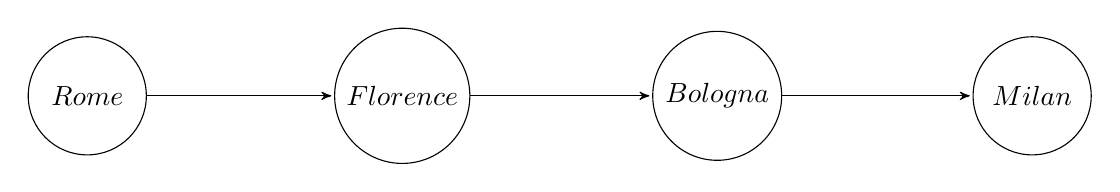
\begin{tikzpicture}[>=stealth',shorten >=1pt,auto,node distance=4cm, state/.style={circle, draw, minimum size=1.5cm}]
				\node[state] 		 (Rome)          {$Rome$};
				\node[state]         (Florence) [right of=Rome]   {$Florence$};
				\node[state]         (Bologna) [right of=Florence]       {$Bologna$};
				\node[state]         (Milan) [right of=Bologna]      {$Milan$};


				\path[->] (Rome)   edge 			node {}   (Florence)
						  (Florence)	edge 			node {}   (Bologna)
						  (Bologna)	edge 			node {}   (Milan);
						
			\end{tikzpicture}
		\end{figure}
		\\
		We will use $b_{ij} i<j$ to express the number of people willing to go from i to j and $f_{ij} i<j$ to express the ticket price for going from i to j. \\
		Our goal is to model the problem such that it could be treated as a minimum-cost flow problem.

	\section{Solution}
		I thought to model the problem as follows:
		\begin{figure}[ht!]
		\centering
		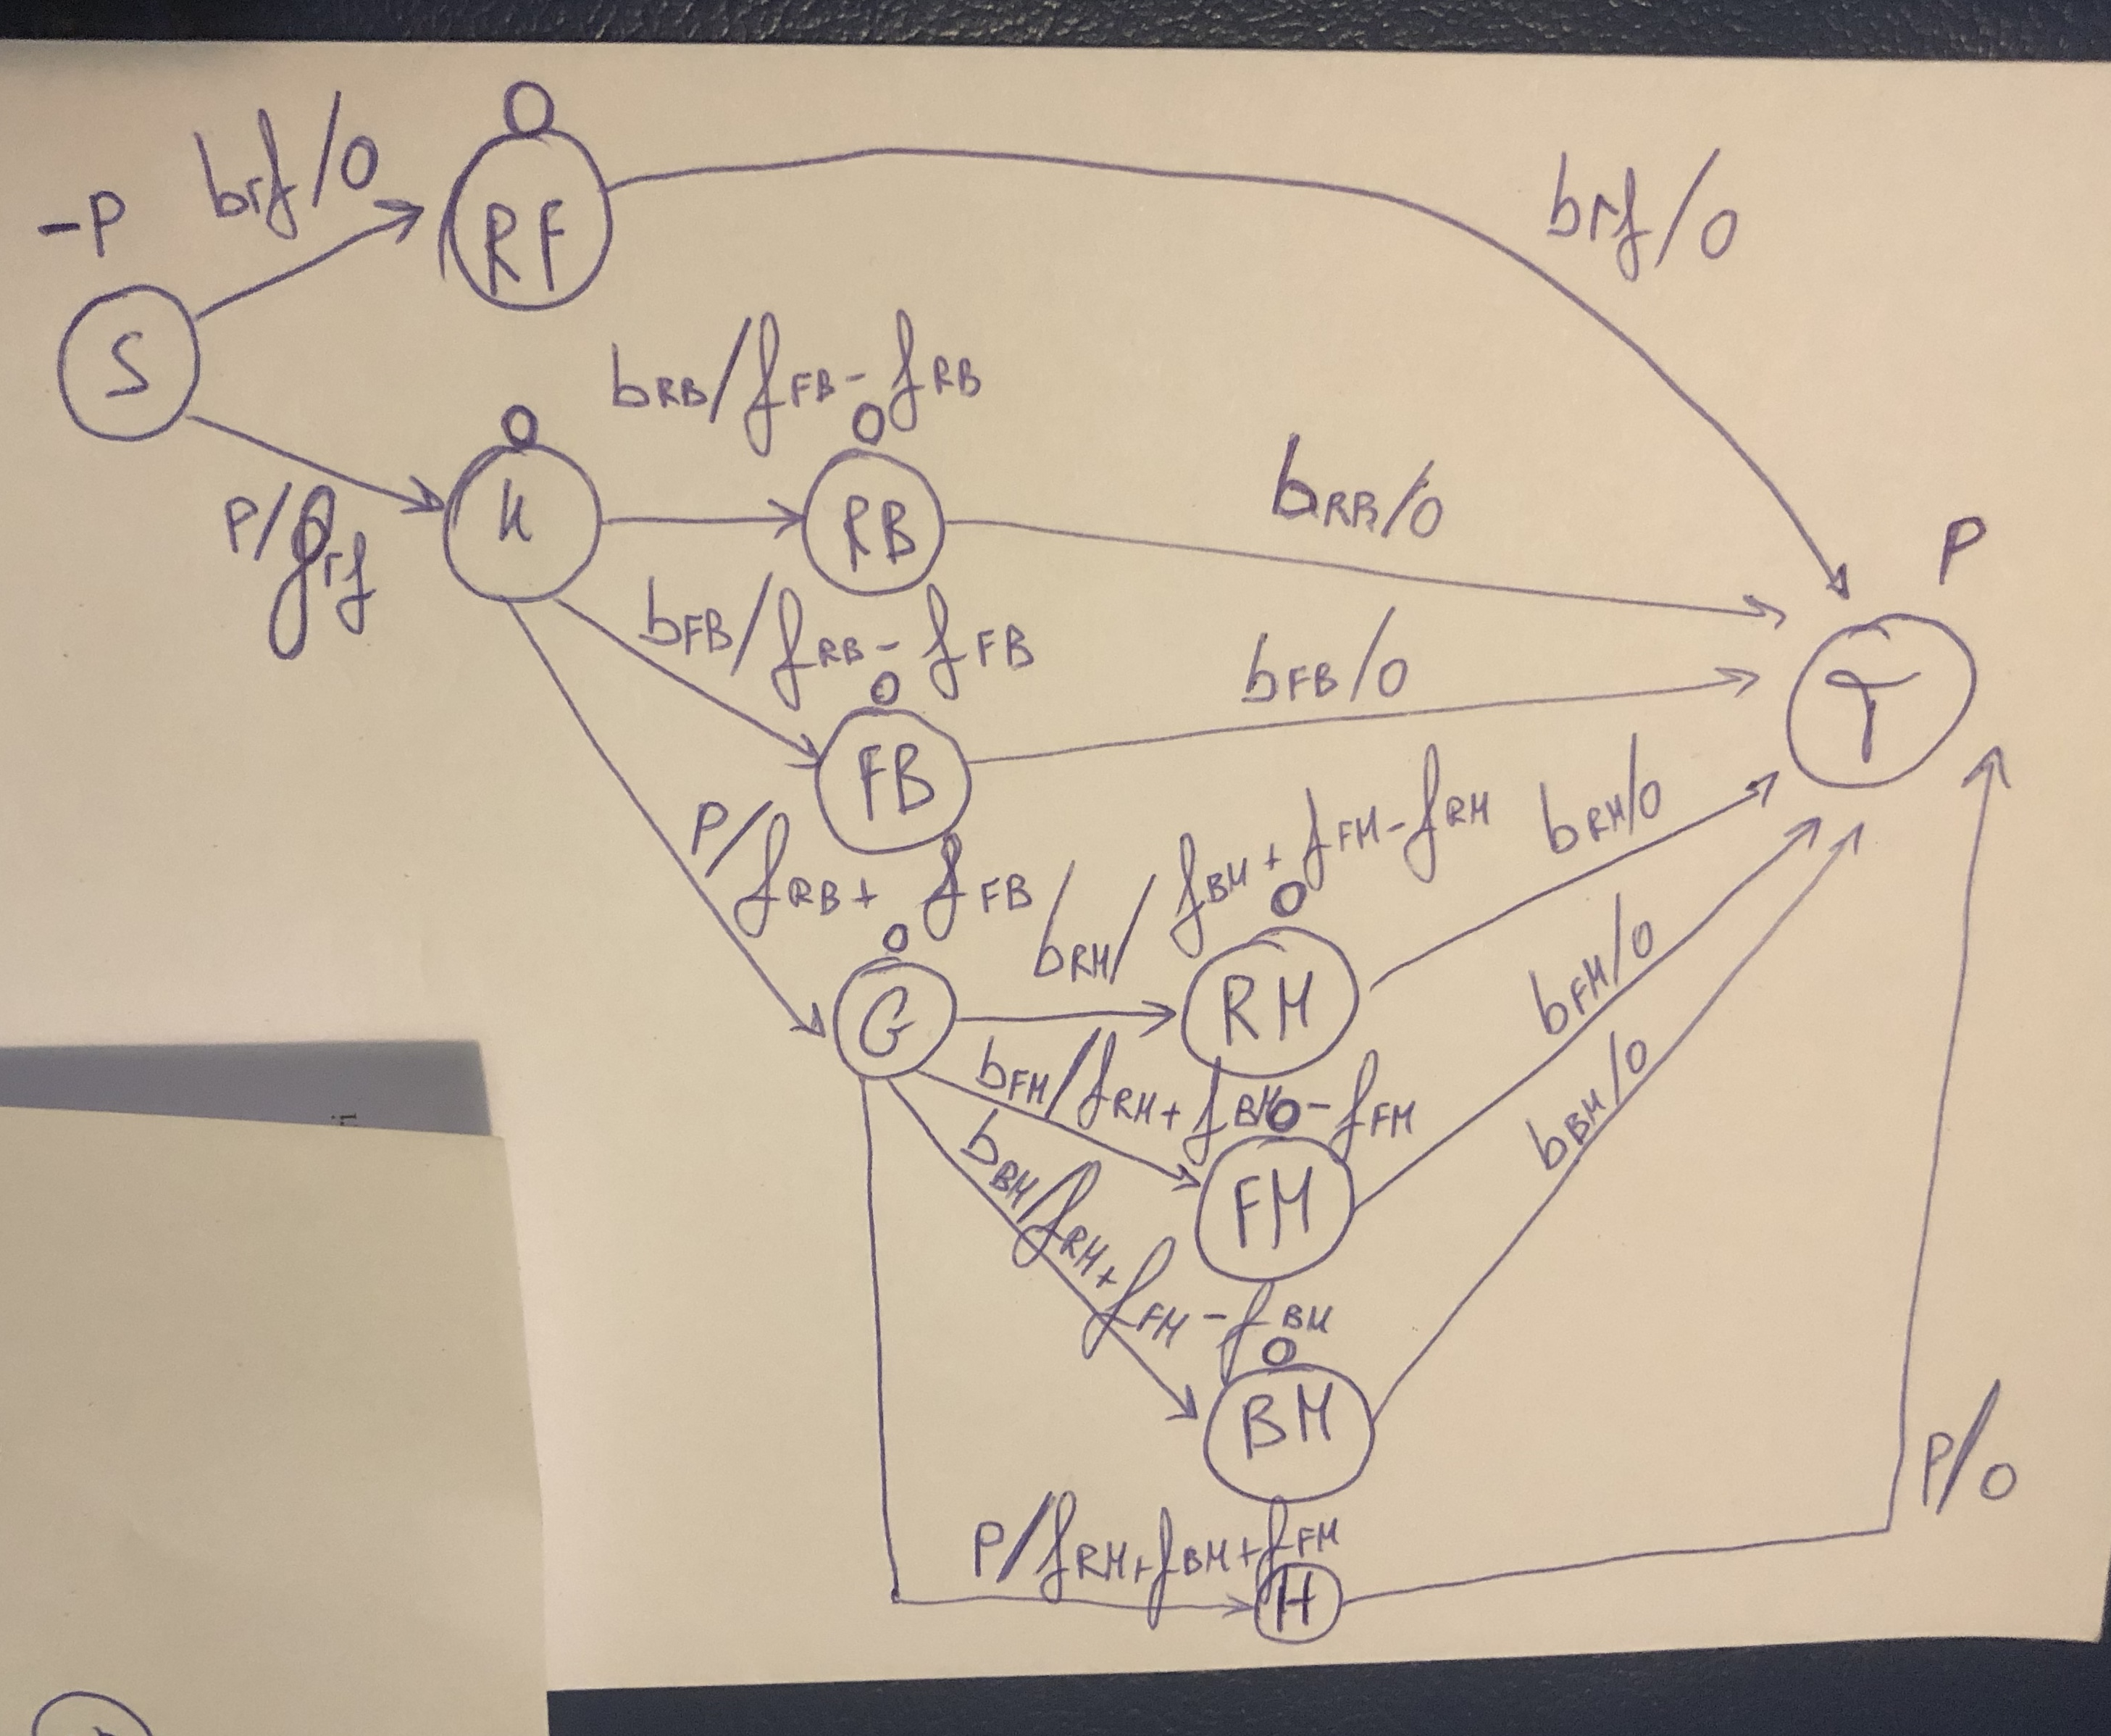
\includegraphics[width=90mm]{graph.JPG}
		\end{figure}

		The idea is to divide into columns the order of arrival in the possible cities and let the flow be at most P at every cut. \\
		Every node is named after the route it represents.\\
		Nodes $K, G, H$ are special nodes used to express the fact that people can show up directly at a station without travelling with our company.\\
		I introduce two nodes, $s$ and $t$ that are the source and the sink of the flow of passengers. On each arch it is specified the capacity $c$ and the cost. I'll use $F(x,y)$ when referring to the flow from node $x$ to node $y$. $N$ is the set of all the nodes. We have the following properties: 
		\begin{itemize}
		\item $\sum_{n \in N} F(x,n) = 0$  $\forall x != s,t$
		\item $\sum_{n \in N} F(s,n) = P = \sum_{n \in N} F(n,t)$ 
		\end{itemize}
		Furthermore, as usual, the flow between two nodes can't be greater than the capacity of the arch that links them.\\
		The cost of each arch represents the money lost for every person that is not taken the other routes "in the same column". \\
		The problem can now be solved as a minimum-cost flow problem.
\end{document}